\section{运动路程和时间的计算}\label{sec:3-5}

一个做匀速直线运动的物体,如果我们知道了它的速度,很容易求出它在一定时间内通过的路程。

例如,做匀速直线运动的物体的速度是 30 米/秒,那么,从计时开始,经过 1 秒,物体通过的路程就是 30 米。
经过 2 秒,物体通过的路程就是 2 个 30 米,即 60 米。
经过 3 秒,物体通过的路程就是 3 个 30 米,即 90 米。
经过 $t$ 秒,物体通过的路程就是 $t$ 个 30 米。
可见,做匀速直线运动的物体,在时间 $t$ 内通过的路程 $s$,等于速度 $v$ 乘以时间 $t$。用公式来表示就是
\begin{gather}
    s = vt \text{。} \label{eq:lucheng-shijian-1}
\end{gather}

同样地,一个做匀速直线运动的物体,如果我们知道了它的速度,也很容易求出它通过一段路程需要的时间。

假如还是那个速度是 30 米/秒的物体,它通过 180 米的路程,需要多少时间呢?
它每通过 30 米,需要 1 秒钟,180 米中有 6 个 30 米,所以需要 6 秒钟。
可见,用路程 $s$ 除以速度 $v$,就可以得到做匀速直线运动的物体,通过这段路程所需要的时间。
用公式来表示就是
\jiange
\begin{gather}
    t = \dfrac{s}{v} \text{。} \label{eq:lucheng-shijian-2}
\end{gather}

我们在初中一年级的数学中学过 “公式变形”。
上面的公式 \eqref{eq:lucheng-shijian-1} 和 \eqref{eq:lucheng-shijian-2},
也可以从匀速直线运动的基本公式 $v = \dfrac{s}{t}$,利用公式变形来直接得出。
公式变形的方法在物理学中经常要用到,希望同学们注意。

\liti 在建设中经常要用到爆破技术。在一次爆破中,用了一条 96 厘米长的引火线来使装在钻孔里的炸药爆炸。
引火线燃烧的速度是 0.8 厘米/秒,点火者点着引火线以后,以 5 米/秒的速度跑开,
他能不能在爆炸前跑到离爆炸地点 500 米远的安全地区?

求出引火线烧完所需的时间 $t$,就可以算出在这段时间内点火者能够跑开的距离,把这个距离同 500 米相比较,
就可以知道点火者是否来得及跑到安全地区。

\jie 用 $s_1$、$v_1$、$t$ 分别表示引火线的长度、燃烧的速度和烧完所需要的时间,
用 $v_2$、$s_2$ 分别表示点火者跑开的速度和在时间 $t$ 内跑开的距离。

引火线烧完所需的时间
$$ \qquad t = \dfrac{s_1}{v_1} = \dfrac{96\text{厘米}}{0.8 \text{厘米/秒}} = 120 \text{秒。} $$

在这段时间内点火者能跑开的距离
$$ s_2 = v_2\;t = 5 \text{米/秒} \times 120 \text{秒} = 600 \text{米。} $$
$$ 600 \text{米} > 500 \text{米。} $$

答:点火者能在炸药爆炸前跑到安全区。

\lianxi

\begin{wrapfigure}[9]{r}{5cm}
    \centering
    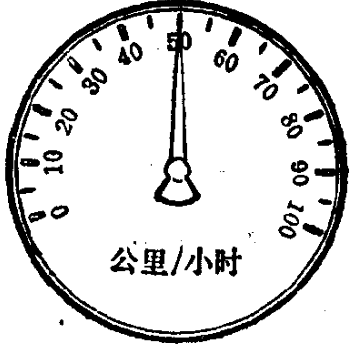
\includegraphics[width=4cm]{../pic/czwl1-ch3-4}
    \caption{}\label{fig:3-4}
\end{wrapfigure}

(1) 汽车司机座前面安装着速度计,它可以指出汽车的行驶速度。
如果速度计的指针如图 \ref{fig:3-4} 所示,汽车用这个速度行驶,经过 45 分钟能够驶出多远?

(2) 南京长江大桥,上层公路桥全长 4589 米。一辆汽车以 36 千米/小时的速度在公路上行驶,
汽车通过公路桥要用多长时间?

(3) 南京长江大桥,下层铁路桥全长 6772 米,其中的江面正桥长 1577 米。
一列火车通过江面正桥用了 2 分钟,这列火车以这样的速度行驶,通过整个铁路桥要多长时间?

(4) 根据天气预报,台风中心以 20 千米/小时的速度向某地接近,台风中心现距该地 150 千米,
预计多长时间后将到达该地。

(5) 测出你用正常速度步行 100 米用的时间,算出步行的速度,再测出你沿学校操场走一圈所用的时间,
算出操场的周长。

(6) 向月球发射的无线电波到达月球并从月球返回地球共需 2.56 秒。
无线电波的传播速度是 $3 \times 10^8$ 米/秒,求月球与地球间的距离。

(7) 光的传播速度是 $3 \times 10^8$ 米/秒,太阳到地球的距离是 $1.5 \times 10^{11}$ 米,
太阳发出的光到达地球需要多长时间?

